\documentclass[12pt, letterpaper]{article} 

\usepackage{amsmath, amssymb, amsthm, enumerate, graphicx}

\title{MATH 189 HW 2}
\author{Dani Nguyen}
\date{Winter 2025}

\begin{document}
\maketitle
\graphicspath{ {./} }

\noindent \textbf{Question 1}
\begin{enumerate}[a.]
    \item Since IQ and GPA is fixed, we will denote those values as a constant $C$
    \begin{align*}
        Y &= C + 35X_3 - 10X_5 \\
        &= C + \mathbb{I}\{\text{has college}\} (35-10X_5)
    \end{align*}
    When fixing IQ and GPA, the model predicts that college graduates will earn less 
    if their GPA is higher than 3.5. Therefore, option iii. is correct.
    \item For a college graduate with IQ 110 and GPA 4.0,
    \begin{align*}
        Y &= 50 + 20(4.0) + 0.07(110) + 35(1) + 0.01(4.0 \cdot 110) - 10(4.0\cdot1) \\
        &= 137.1 \text{ thousand dollars}
    \end{align*}
    \item False, because GPA and IQ are on average very large numbers, especially 
        when multiplied, that even a low coefficient can lead to large effects in
        salary. This does not mean that there is little evidence of an interaction 
        effect, one would need to look at the $p$-values of the interaction term to 
        know whether there exists an interaction effect. 
\end{enumerate}
\newpage
\noindent \textbf{Question 2} \\
\begin{align*}
    \hat y_i &= x_i \hat \beta \\
    &= x_i \frac{\sum_{i=1}^{n}x_iy_i}{\sum_{i'=1}^{n}x_{i'}^2} \\
    &= \frac{\sum_{i=1}^{n}x_i^2 y_i}{\sum_{i'=1}^{n}x_{i'}^2} \\
    &= \sum_{i=1}^{n} \frac{x_i^2}{\sum_{i'=1}^{n}x_{i'}^2} y_i
\end{align*}
Let $a_i = \frac{x_i^2}{\sum_{i'=1}^{n}x_{i'}^2}$
\begin{align*}
    \hat y_i = \sum_{i=1}^{n}a_iy_i
\end{align*}

\noindent \textbf{Question 3} \\ \\
Recall that $\beta_0 = \bar y + \beta_1 \bar x$. This can be rearranged to 
$\bar y = \beta_0 - \beta_1\bar x$. This means that the equation for simple linear 
regression is centered at and will always pass through the point $(\bar x, \bar y)$. \\

\noindent \textbf{Question 4}
\begin{align*}
    R^2 &= \frac{TSS-RSS}{TSS} \\
    &= \frac{\sum_{i=1}^{n}(y_i)^2 - \sum_{i=1}^{n}(y_i - \hat\beta_0 -\hat\beta_1x_i)^2}{\sum_{i=1}^{n}(y_i)^2} \\
    &= \frac{\sum_{i=1}^{n}(y_i)^2 - \sum_{i=1}^{n}(y_i)^2 + \frac{\Big[ \sum_{i=1}^{n} (x_i - \bar x)(y_i - \bar y)\Big]^2}{\sum_{i=1}^{n} (x_i - \bar x)^2}}{\sum_{i=1}^{n}(y_i)^2} \\ 
    &= \frac{\sum_{i=1}^{n}(x_iy_i)^2}{\sum_{i=1}^{n}(x_i)^2 \sum_{i=1}^{n}(y_i)^2}\\
    R &= \frac{\sum_{i=1}^{n}(x_iy_i)}{\sum_{i=1}^{n}(x_i) \sum_{i=1}^{n}(y_i)} = \frac{Cov(X_iY_i)}{Var(X_i)^\frac 12 Var(Y_i)^\frac 12}
\end{align*} 
\newpage
\noindent \textbf{Question 5} 
\begin{enumerate}
    \item[c.] Length of the vector $y$ is $11.62$. In this linear model $\beta_0$ is $-1$ and $\beta_1$ is $0.5$.
    \item[d.] The distribution is linear, positive, and moderately spread out.
    \item[e.] The model is linear and has positive slope, $\hat \beta_1$ is 0.49214551 and $\hat\beta_0$ is -1.01900639 which is fairly close to our $\beta_1$ of 0.5 and $\beta_0$ of -1
    \item[f.] 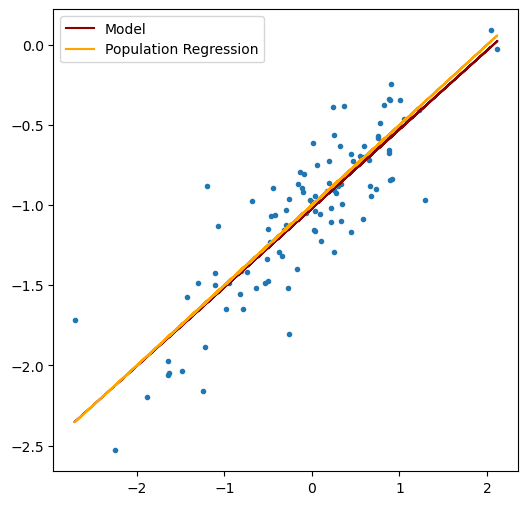
\includegraphics{q5f.png} 
    \newpage
    \item[g.] The quadratic line of best fit seems to fit just as well as the linear model, although there is no evidence that it improves the fit. \\ 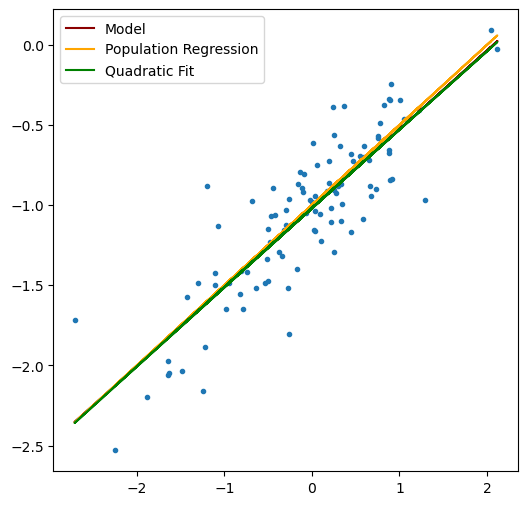
\includegraphics{q5g.png} \newpage
    \item[h.] The points are much closer to the least squares regression line, and the differences between the model and the population regression decreases \\ 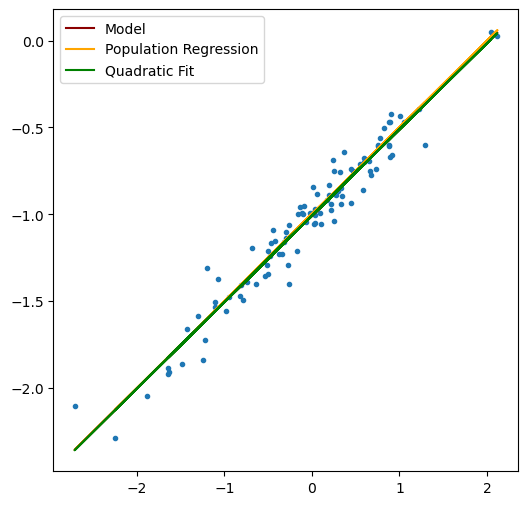
\includegraphics{q5h.png} \newpage
    \item[i.] The points are more spread out along the least squares regression line, and the differences between the model and the population regression increases \\ 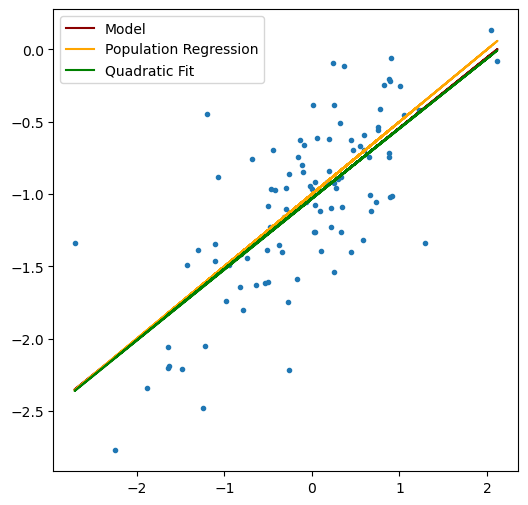
\includegraphics{q5i.png}
    \item[j.] For the noisy dataset, the confidence interval for $\beta_0$ is $\left[-1.03 \pm 0.0798\right]$, $\beta_1$ is $\left[0.4874 \pm 0.0933\right]$. \\
            For the original dataset the confidence interval for $\beta_0$ is $\left[-1.02 \pm 0.0499\right]$, $\beta_1$ is $\left[0.4921 \pm 0.0584\right]$. \\
            For the less noisy  dataset the confidence interval for $\beta_0$ is $\left[-1.007 \pm 0.0200\right]$, $\beta_1$ is $\left[0.4969 \pm 0.0233\right]$. 
\end{enumerate}
\newpage
\noindent \textbf{Question 6}
\begin{enumerate}[a.]
    \item None of the distributions seem to fit a linear regression model, but all of the predictors have p-value below 0.05 when fitted with crime rate per capita data aside from chas, which has a p-value of 0.209\\
    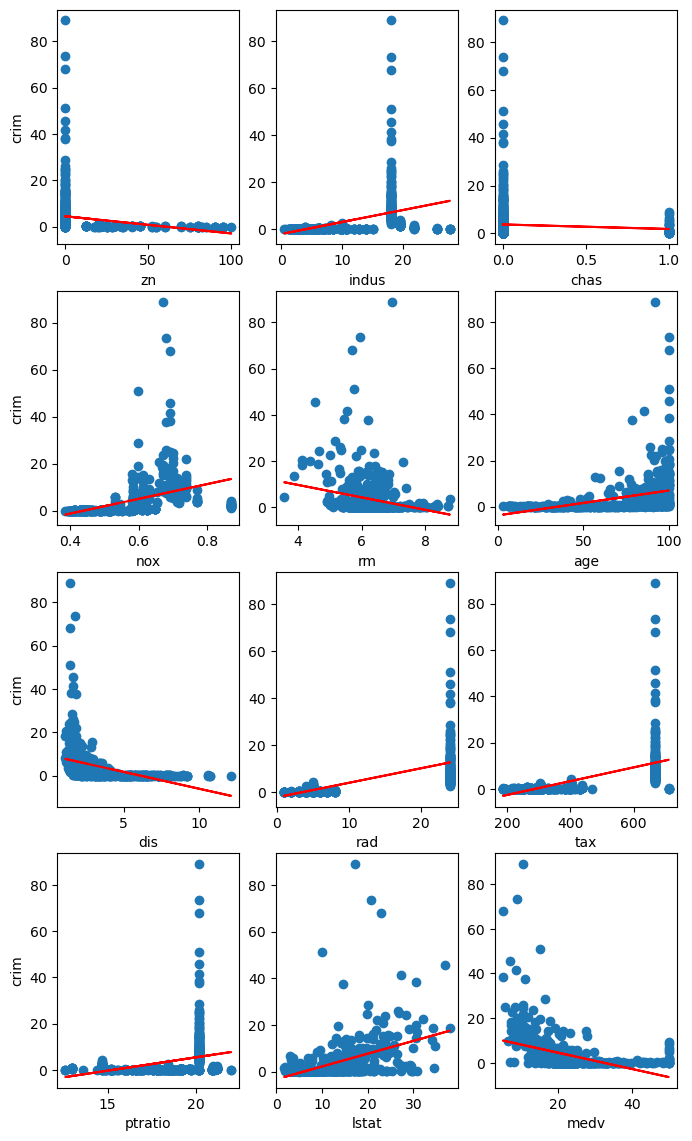
\includegraphics[scale=0.5]{q6a.png}
    \newpage
    \item 
\begin{table}[h]
\centering
\begin{tabular}{l r r r r}
\hline
& \textbf{coef} & \textbf{std err} & \textbf{t} & \textbf{P$>|$t$|$} \\
\hline
intercept & 13.7784 & 7.082 & 1.946 & 0.052 \\
zn & 0.0457 & 0.019 & 2.433 & 0.015 \\
indus & -0.0584 & 0.084 & -0.698 & 0.486 \\
chas & -0.8254 & 1.183 & -0.697 & 0.486 \\
nox & -9.9576 & 5.290 & -1.882 & 0.060 \\
rm & 0.6289 & 0.607 & 1.036 & 0.301 \\
age & -0.0008 & 0.018 & -0.047 & 0.962 \\
dis & -1.0122 & 0.282 & -3.584 & 0.000 \\
rad & 0.6125 & 0.088 & 6.997 & 0.000 \\
tax & -0.0038 & 0.005 & -0.730 & 0.466 \\
ptratio & -0.3041 & 0.186 & -1.632 & 0.103 \\
lstat & 0.1388 & 0.076 & 1.833 & 0.067 \\
medv & -0.2201 & 0.060 & -3.678 & 0.000 \\
\hline
\end{tabular}
\caption{OLS Regression Results for Boston Crime Data}
\label{tab:boston_regression}
\end{table}

We can reject the null hypothesis $H_0 = \beta_j =0$ 
for zn, dis, rad, and medv as they have P $>$ $|t|$ less than 0.05.

\item The $\beta_j$ values are mostly similar, aside from nox, which is wildly different between multivariate (-9.9576) and simple linear regression (31.2485) \\ 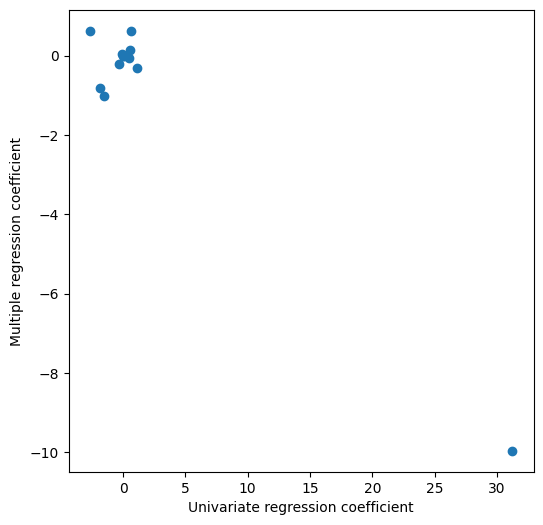
\includegraphics[scale=0.5]{q6c.png}
\item 
\end{enumerate}
\end{document}